\part{A Multi-Agent System for Continuous Optimization}

\chapter{Agent-Based Modeling and Simulation of a Continuous Optimization Problem}

[[Insister sur le découpage inhérent au problème (pas de réductionnisme)]]
[[utiliser un exemple en fil rouge -> Turbofan ?]]

\section{Problem Modeling with NDMO}\label{modeling}

[[A CHANGER: In answer to the previous shortcomings, we propose a generic approach called Natural Domain Modeling for Optimization (NDMO) that relies on a natural or intrinsic description of the problem (\textit{i.e.} close to the reality being described).]]

\begin{figure}[]
	\centering
	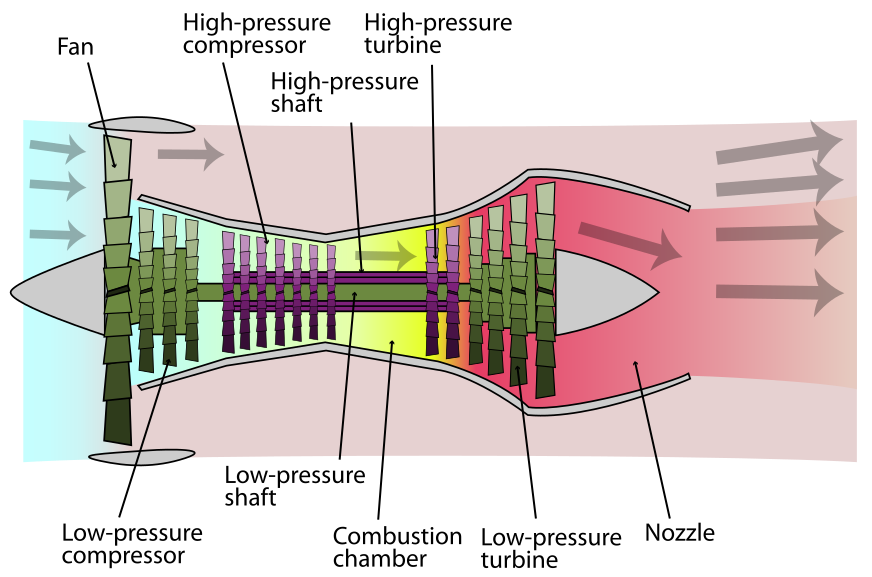
\includegraphics[width=0.8\textwidth]{Turbofan_operation}
	\caption{Illustration of a Turbofan engine (CC SA-BY  \href{http://en.wikipedia.org/wiki/File:Turbofan_operation.svg}{K. Aainsqatsi})}
	\label{turbofan_illu}
\end{figure}

To illustrate how an optimization problem is modeled, we use a simplified Turbofan optimization problem. On \figurename{} \ref{turbofan_illu}, an illustration of the principle of the turbofan can be seen. In this figure, the bypass ratio is the ratio between the air drawn in by the fan not entering engine core (which is \emph{bypassed}) and the air effectively used for the combustion process. The pressure ratio is the ratio between pressure produced by the compressors and the pressure it receives from the environment.

In order to identify the elements of a generic continuous optimization model, we worked with experts from several related fields: numerical optimization, mechanics as well as aeronautics and engine engineers. As a result, we identified five classes of interacting entities: \emph{models}, \emph{design variables}, \emph{output variables}, \emph{constraints} and \emph{objectives}. These entities and their relations are represented by the diagram in \figurename{} \ref{class_diag}, that we detail next.

\begin{figure}[t]
	\centering
	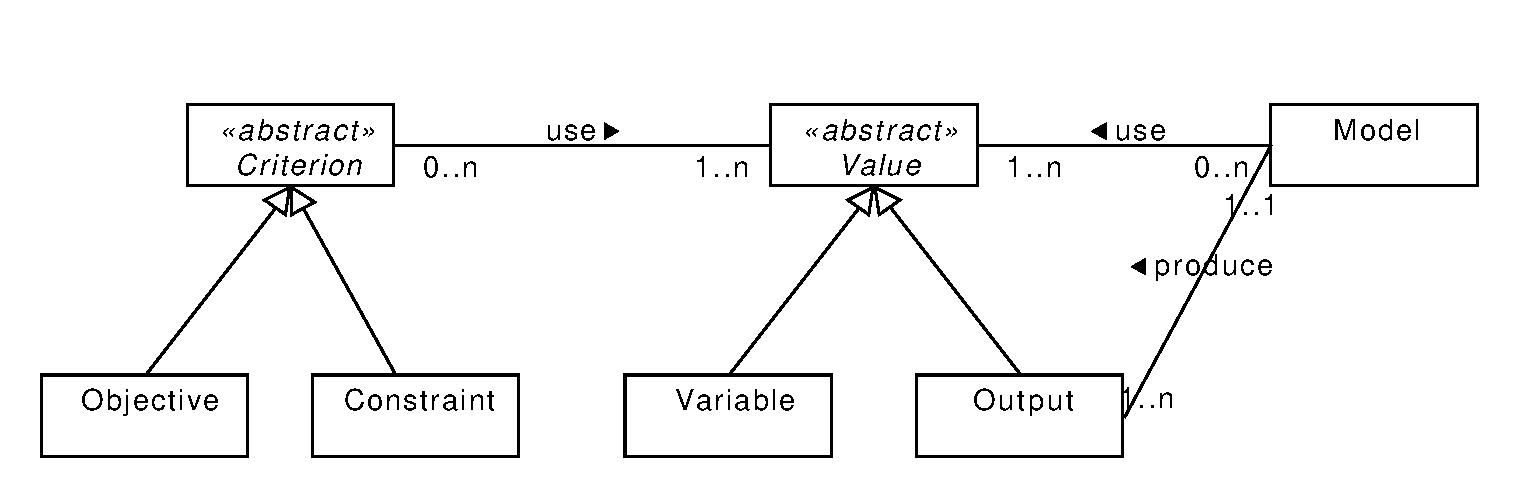
\includegraphics[width=0.9\textwidth]{class_diag}
	\caption{Class diagram of MDO problems}
	\label{class_diag}
\end{figure}

In \figurename{} \ref{turbofan:math}, the analytic expression of this optimization problem is given, while in \figurename{} \ref{turbofan:graph}, the problem is presented as a graph of the different entities. The design variables of this problem are $pi\_c$ and $bpr$, which indicate respectively the compressor pressure ratio and the bypass ratio of the engine. The turbofan model produces three outputs: $Tdm0$, $s$ and $fr$, representing respectively the thrust, fuel consumption and thrust ratio of the engine. In this problem we try to maximize the thrust and minimizing the fuel consumption while satisfying some feasibility constraints. 

\begin{figure}[]
\centering
	\begin{subfigure}[b]{0.4\textwidth}
		$\begin{array}{c}
			(Tdm0, s, fr) = Turbofan(pi\_c, bpr) \\
			max \; Tdm0 \\
			min \; s \\
			subject \; to \\
			s \leq 155 \\
			fr \geq 4
		\end{array}$
		\caption{mathematical formulation.}\label{turbofan:math}
	\end{subfigure}
	\hfill%
	\begin{subfigure}[b]{0.55\textwidth}
			\centering
			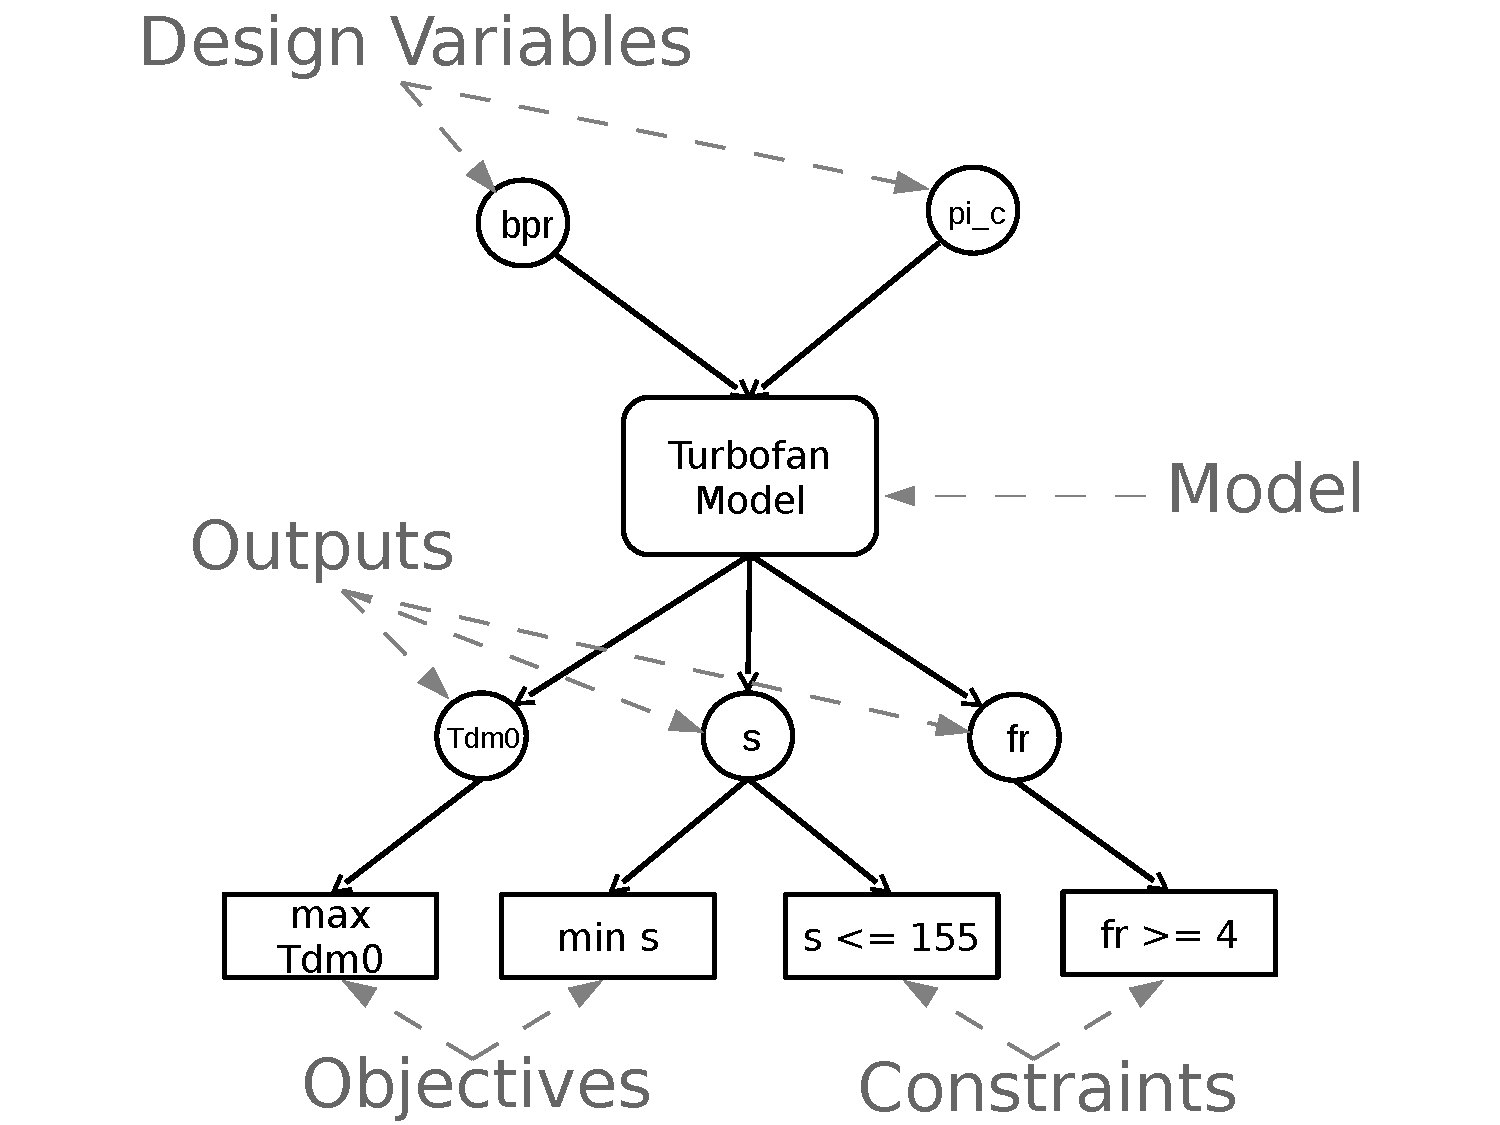
\includegraphics[width=\textwidth]{testcases-Turbofan-annoted}
			\caption{corresponding entities graph.}\label{turbofan:graph}
	\end{subfigure}

\caption{Turbofan problem.}
\label{turbofan}

\end{figure}

Let's now see in more details the roles of each of these fives entities: \emph{model}, \emph{variable}, \emph{output}, \emph{constraint} and \emph{objective}.

\subsubsection*{Models.}

[[DIRE QU'UN MODELE CORRESPOND A UN NIVEAU D'ABSTRACTION ARBITRAIRE (PEUT ETRE UNE DISCIPLINE ENTIERE)]]

In the most general case, a \emph{model} can be seen as a black box which takes input values (which can be \emph{design variables} or \emph{output variables}) and produces output values. A \emph{model} represents a technical knowledge of the relations between different parts of a problem and can be as simple as a linear function or a much more complex algorithm requiring several hours of calculation. Often some properties are known (or can be deduced) about a model and specialized optimization techniques can exploit this information.
In our Turbofan example, a \emph{model} entity is the $Turbofan$ function which calculate the three outputs using the values of $bpr$ and $pi\_c$.

\subsubsection*{Design Variables.}

These are the inputs of the problem and can be adjusted freely (within their defining boundaries). The goal is to find the set(s) of values for these variables that maximize the objectives while satisfying the constraints.
\emph{Design variables} are used by \emph{models} to calculate their outputs and by constraints and objectives to calculate their current value. A \emph{design variable} can be shared among several \emph{models}, objectives and constraints.
Keeping with our example, $bpr$ and $pi\_c$ are the two \emph{design variables} of our optimization problem.

\subsubsection*{Output Variables.}

These values are produced by a \emph{model}, and consequently cannot be changed freely.
As for the \emph{design variables}, the \emph{output variables} are used by \emph{models} to calculate their outputs and by constraints and objectives to calculate their current value.
In our example, $Tdm0$, $s$ and $fr$ are \emph{output variables} produced by the $Turbofan$ model.

\subsubsection*{Constraints.}

These are strict restrictions on some parts of the problem, represented as functional constraints defined by equalities and/or inequalities. These can be the expression of a physical constraint, or a requirement concerning the problem.
Regarding the Turbofan, the two \emph{constraints} are $s <= 155$ and $fr >=4$.

\subsubsection*{Objectives.}

The goals to be optimized. In the general case, different objectives are often contradictory.
The two \emph{objectives} of the Turbofan problems are to maximize $Tdm0$ and to minimize $s$.

Constraints and objectives are usually regrouped under the more general term of optimization criteria. 

\paragraph*{}
An interesting and important point is that both models, constraints and objectives involve computation. Often the most heavyweight calculus is encapsulated inside a model and the calculi concerning criteria tend to be simple equations, but this is neither an absolute requirement nor a discriminating characteristic.

The NDMO modeling aims to provide the most complete and natural representation of the problem. This modeling preserves the relations between the domain entities and is completely independent of the solving process. 

[[SAY IT IS A BIPARTITE GRAPH BETWEEN VALUES ENTITIES AND INTERNAL MODEL ENTITIES]]

\section{From an Optimization Problem to a Multi-Agent System}

Based on the NDMO modeling in section \ref{modeling}, we propose a multi-agent system where each domain entity is associated with an agent. Thus the multi-agent system is the representation of the problem to be solved with the links and communication between agents reflecting the natural structure of the problem. It is worth underlining the fact that this transformation (\textit{i.e.} the agentification) can be completely automatic as it is fully derived from the expression of the problem.

\begin{figure}
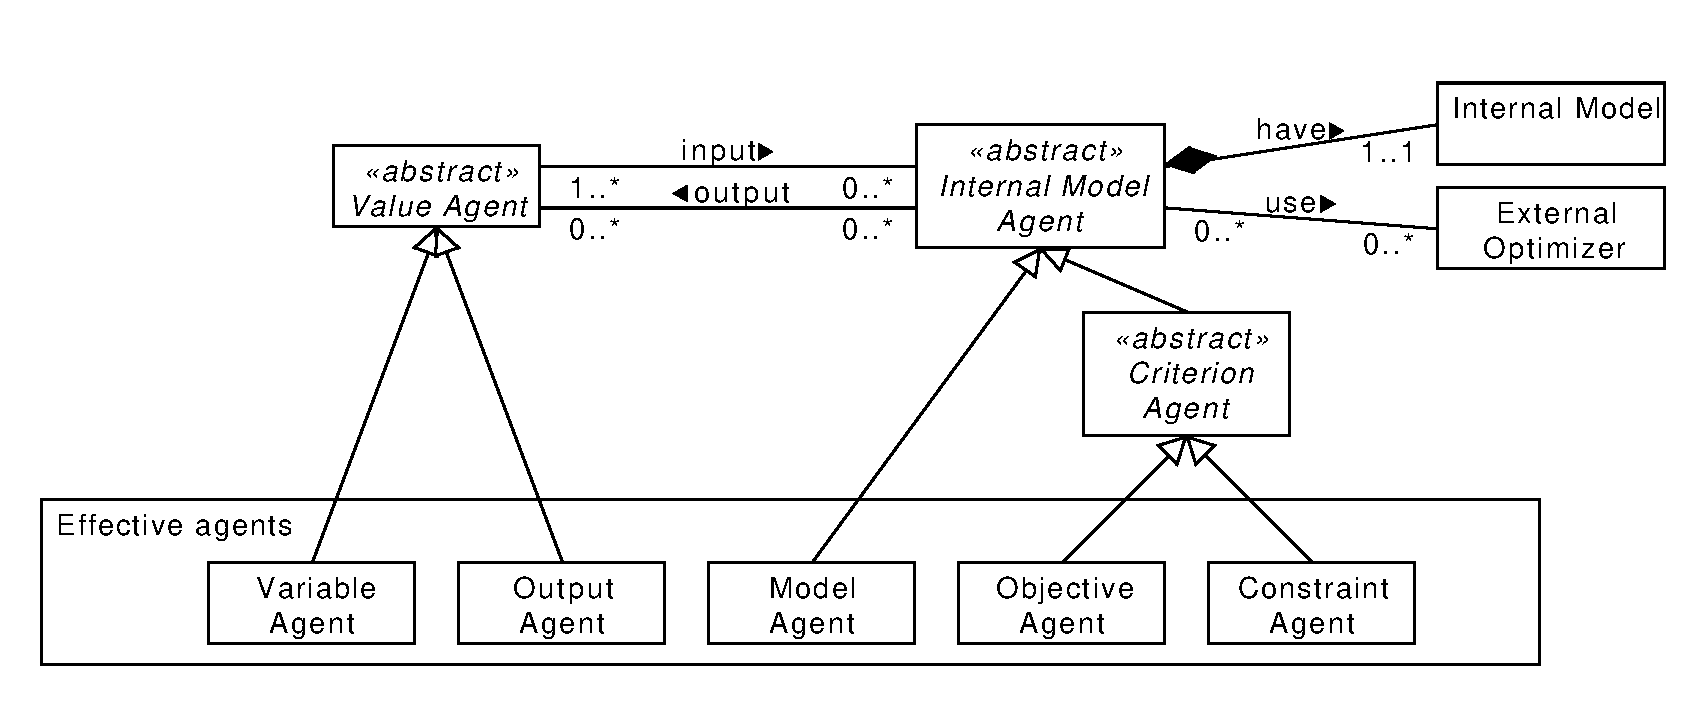
\includegraphics[width=\textwidth]{agent_class_diag}
\caption{System class diagram}\label{SMA_class_diagram}

\end{figure}

The solving process - constituted by the collective behavior of the agents - basically relies, on change-value requests sent by the criteria agents resulting in cooperatively decided adjustments done by the \emph{design variables} and on new values computed by the models resulting on the satisfaction or dissatisfaction of the criteria agents. 
In the same way we presented the different elements of NDMO, we now detail the behaviors of our five agent types: \emph{model}, \emph{variable}, \emph{output}, \emph{constraint} and \emph{objective} agents.
A summary of the basic principles of each agent type is given in Algorithm \ref{agent_algo}.

\subsubsection*{Model Agent.}

A \emph{model agent} takes charge of a model of the problem. It interacts with the agents handling its inputs (which can be \emph{variable} or \emph{output agents}) and the \emph{output agents} handling its outputs. Its individual goal is to maintain the consistency between its inputs and its outputs. To this end, when it receives a message from one of its inputs informing it of a value change, a \emph{model agent} recalculates the outputs values of its model and informs its\emph{output agents} of their new value. On the other part, when a \emph{model agent} receives a message from one of its \emph{output agents} it translates and transmits the request to its inputs. 

To find the input values corresponding to a specific desired output value, the \emph{model agent} uses an external optimizer. This optimizer is provided by the engineer based on expert domain-dependent knowledge regarding the structure of the model itself.
It is important to underline that the optimizer is used only to solve the local problem of the \emph{model agent}, and is  not used to solve the problem globally.


%\begin{algorithm}
%\caption{Behavior of a Model Agent}
%\begin{algorithmic}
%\While{running}
%	\State Receive Messages
%	\If{received new informs}
%        \State recalculate outputs
%        \State inform output agents
%    \EndIf      
%	\If{received new requests}
%       \State  use optimizer to find adequate inputs
%        \State propagate requests to input agents
%    \EndIf
%\EndWhile
%\end{algorithmic}
%\end{algorithm}

\subsubsection*{Variable Agent.}

This agent represents a \emph{design variable} of the problem. Its individual goal is to find a value which is the best equilibrium among all the requests it can receive (from models and criteria for which it is an input). The agents using the variable as input can send to it request asking to change its value. When changing value, the agent informs all agents linked to it of its new value. 

%\begin{algorithm}
%\caption{Behavior of a Variable Agent}
%\begin{algorithmic}
%\While{running}
%	\State Receive Messages  
%	\If{received new requests}
%       \State select most important
%       \State adjust value
%       \State inform related agents
%    \EndIf
%\EndWhile
%\end{algorithmic}
%\end{algorithm}

\subsubsection*{Output Agent.}
The \emph{output agent} takes charge of an output of a model. \emph{Output agent} and \emph{variable agents} have similar roles, except \emph{output agents} cannot directly change their value. Instead they send a request to the \emph{model agent} they depend on. In this regard, the \emph{output agent} act as a filter for the \emph{model agent} it depends on, selecting among the different requests the ones it then transmits.

%\begin{algorithm}
%\caption{Behavior of an Output Agent}
%\begin{algorithmic}
%\While{running}
%	\State Receive Messages
%	\If{received new informs}
%        \State update its value
%        \State inform related agents
%    \EndIf      
%	\If{received new requests}
%       \State  select most important
%        \State transmit selected request to model agent
%    \EndIf
%\EndWhile
%\end{algorithmic}
%\end{algorithm}

As we will see in the next section, the \emph{output agent} is distinct from the \emph{variable agent} in the way that it can be involved in cycles. A cycle is a situation of interdependent models (that is, models which depend of each other to calculate their outputs).

%We describe in the next section the main difficulties when solving an optimization problem including interdependencies, and how can an \emph{output agent} detect and handle them.

\subsubsection*{Constraint Agent.}
 \emph{The constraint agent} has the responsibility for handling a constraint of the problem. When receiving a message from one of its inputs, the agent recalculates its constraint and checks its satisfaction. If the constraint is not satisfied, the agent sends \emph{change value} requests to its inputs.

%\begin{algorithm}
%\caption{Behavior of a Constraint/Objective Agent}
%\begin{algorithmic}
%\While{running}
%	\State Receive Messages
%	\If{received new informs}
%        \State update its value
%        \State use optimizer to find adequate inputs
%        \State send new requests to input agents
%    \EndIf      
%\EndWhile
%\end{algorithmic}
%\end{algorithm}

It should be noted that, to estimate the input values required to satisfy the constraint on its computed value, this agent employs the same technique as the \emph{model agent} (\textit{i.e.} an external optimizer).

\subsubsection*{Objective Agent.}
The  \emph{objective agent} is in charge of an objective of the problem. This agent sends requests to its inputs aiming to improve its objective, and recalculates the objective when receiving  \emph{value changed} messages from its inputs.

This agent uses an external optimizer to estimate input values which would improve the objective, as the model and constraint agents.


\chapter{Agents Behavior}

We will now discuss the behavior the the five agent types identified in the previous chapter. The functioning of the system can be divided into two main tasks: problem simulation and collective solving.

Problem simulation can be seen as the equivalent of the analysis of classical MDO method. The agents behavioral rules related to problem simulation concern the propagation of the values of design variables to the models and criteria based on the value. For this part, the agents will exchange \emph{inform} messages which contains calculated values. The \enquote{message flow} is top-down: the initial inform messages will be emitted by the variable agents and will be propagated down to the criteria agents. The illustration of the messages flow of simulation is shown on \figurename{} \ref{messages_flow:inf}.

Collective solving concerns the optimization of the problem. The agent behavioral rules related to collective solving are about satisfying the constraints while improving the objectives. For this part, the agents will exchange \emph{request} messages which contains desired variations of values. The \enquote{message flow} is bottom-up: the initial request messages will be emitted by the criteria agents and propagated up to variable agents. The illustration of the messages flow of solving is shown on \figurename{} \ref{messages_flow:req}.

\begin{figure}[h]
	\begin{subfigure}[b]{0.4\textwidth}
		\centering
		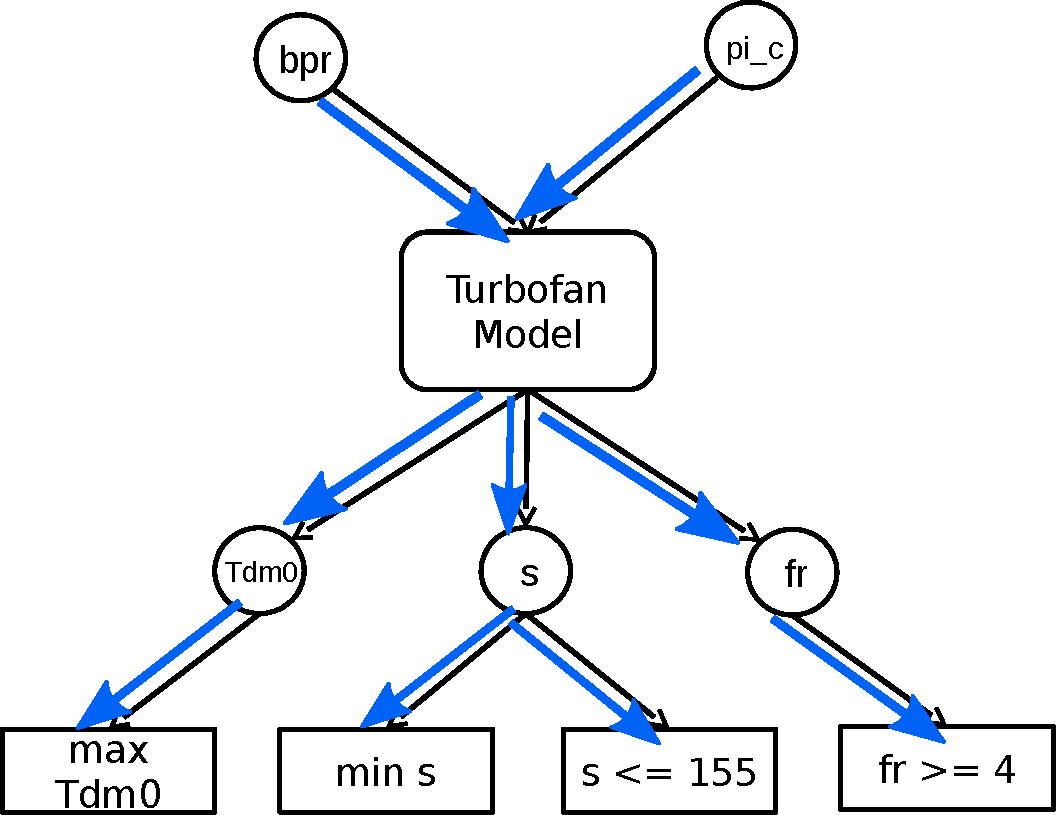
\includegraphics[width=\textwidth]{testcases-Turbofan-informs}
		\caption{Informs flow for simulation}\label{messages_flow:inf}
	\end{subfigure}
	\hfill
  	\begin{subfigure}[b]{0.4\textwidth}
		\centering
		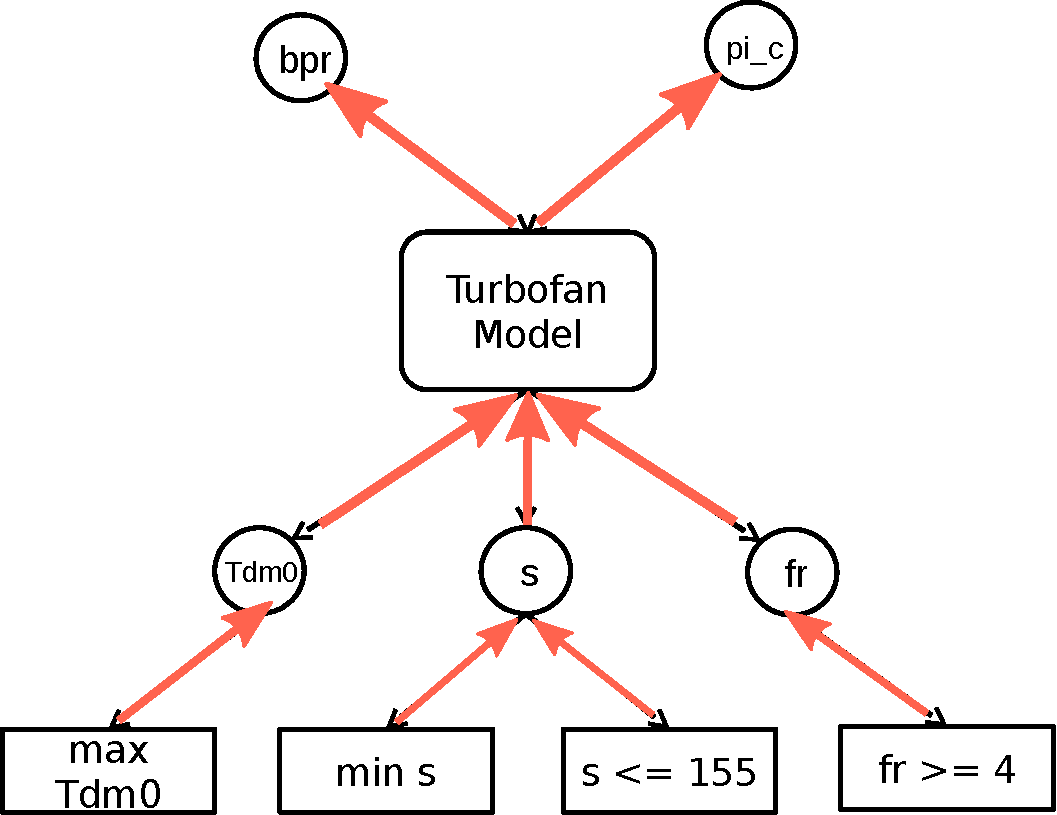
\includegraphics[width=\textwidth]{testcases-Turbofan-requests}
		\caption{Requests flow for solving}\label{messages_flow:req}
	\end{subfigure}

	%new line
	\centering
	 \begin{subfigure}[b]{0.4\textwidth}
		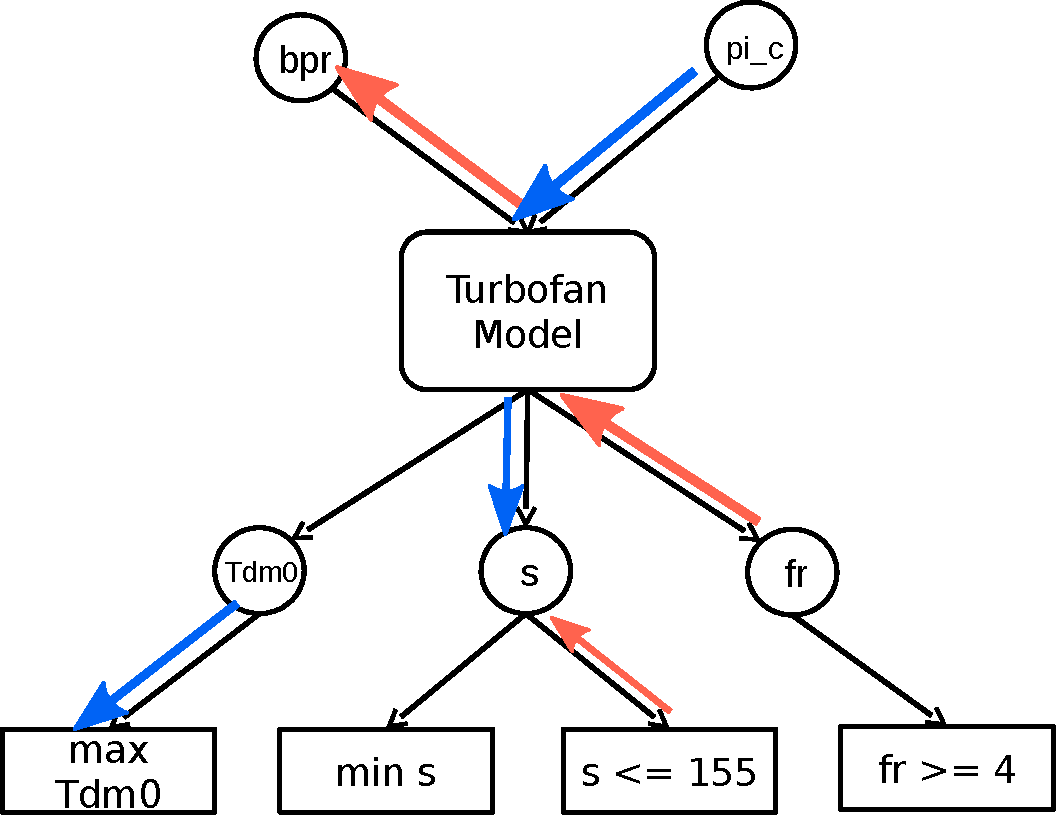
\includegraphics[width=\textwidth]{testcases-Turbofan-informs_requests}
		\caption{Effective messages flow}\label{messages_flow:eff}
	\end{subfigure}
	
	\caption{Messages flow for simulation and solving}
	\label{messages_flow}

\end{figure}

The agents behaviors regarding these two parts can be studied quite independently, we will thus present them separately.  It is however important to remember that these two parts are not executed separately. At runtime the agents will simulate the problem and solve it in parallel. Moreover, the different parts of the system will not necessarily work in a synchronous fashion. The effective messages flow of the system will more probably be akin to the \figurename{} \ref{messages_flow:eff}.

\section{Problem Simulation}

In this section we will present the agents behavior related to the simulation of the problem. Regarding this part, the main concern of the agents is to ensure consistency between the values of the design variables and the produced output. To this end, the agents will propagate \emph{Inform} messages through the system.

An inform message carry a new value $v$. The exact semantic of this information slightly changes depending on which agents are involved:

\begin{itemize}
\item If the message is sent from a value agent (variable or output) to a model or criterion agent, it indicates to the receiving agent that the sending agent has changed value.

\item If the message is sent from a model agent to an output agent, it indicates to the receiving agent that the model has calculated its new value.
\end{itemize}

In practice this distinction is not fundamentally important to understand the functioning of the system.

As stated in section \ref{modeling}, models, constraints and objectives involve a specific calculation operation. For example the constraint $x -y \geq 0$ implies the very basic calculation $x - y$. We regroup these operations under the term \emph{internal models}. As we said, no specific hypothesis is done concerning the nature of an internal model and, more importantly, no distinction is done regarding the internal model used by a model agent and the one used by an objective or a constraint agent.\\
While in some cases specific informations can be known regarding the nature of an internal model, in the most general case these internal models can be seen as black boxes and are handled as such by the agents.

\subsection{Variable Agent}

Regarding problem simulation, the role of the variable agent is to ensure that the agents to which it is connected know its current value.
A variable agent has to send new Inform messages when:
\begin{compactitem}
\item new agents are connected to it (typically at the creation of the system)
\item it decided to change its value based on received requests (see \ref{collective_solv}[[CHANGE TO POINT DIRECTLY TO VARIABLE AGENT]])
\item the designer changed its value
\end{compactitem}

The behavior of the variable agent is summarized in algorithm \ref{algo_simulating_variable}.

\begin{algorithm}
\caption{Problem Simulation - Variable Agent Behavior}
\label{algo_simulating_variable}

	$C \leftarrow$ previously connected agents\;
	$C'\leftarrow$  newly connected agents\;
		
	$v \leftarrow$ previous value\;
	$v'\leftarrow$ new value\;
	
	\tcp{notify contacts of value change}
	\If{$v \neq v'$}{
		$v \leftarrow v'$\;
		\ForEach{agent $a \in C$}{
			send($a$, new Inform($v$))\;
		}
	}
	
	\tcp{send its value to new contacts}
	\If{$C' \neq \emptyset$}{
		\ForEach{agent $a \in C'$}{
			send($a$, new Inform($v$))\;
		}
		$C \leftarrow C + C'$\tcp{memorize new connected agents}
	}
	
\end{algorithm}

\subsection{Model Agent}\label{simulation_model}

A model agent must maintain consistency between its inputs and outputs. When receiving an Inform message from one of the agents controlling its inputs, the model agent reevaluates its internal model taking the new value into account. Using the new values produced by the internal model, the model agents then send Informs messages to the agents responsible of its outputs.

All outputs of a model agent are not necessary associated with an ouput agent. For example, if the designer is not interested by the value represented by one of the outputs, he is not required to represent it by an agent. In this case the model agent will silently calculate the new value of the output at the same time than the others, but will not propagate it\footnote{Remember that the internal model of the agent is a black box, consequently the agent cannot choose to evaluate it partially. If the evaluation of the output could has been done independently from the others, it could be preferable to create two separate models}.

However, as the problem is dynamic, the designer can decide at any time to connect a new output agent to a previously unconnected output. In this case, the model agent must send to the output agent the last value it calculated for this output.

The behavior of the model agent is summarized in algorithm \ref{algo_simulating_model}.

\begin{algorithm}
\caption{Problem Simulation - Model Agent Behavior}
\label{algo_simulating_model}

	$C \leftarrow$ previously connected output agents\;
	$C'\leftarrow$  newly connected output agents\;
	
	$\{v_i\} \leftarrow$ new input values\;
			
	\If{$\{v_i\} \neq \emptyset$}{
		$\{v_o\} \leftarrow$ previous output values\;
		$\{v'_o\}\leftarrow Internal\_Model(\{v_i\})$\tcp{use internal model to recalculate outputs}
		\ForEach{agent $o \in C$}{
			\tcp{inform output agents of their new value}
			send($o$, new Inform($v'_o$))\;
		}
	}
	
	\tcp{Send their value to new outputs}
	\If{$C' \neq \emptyset$}{
		\ForEach{agent $o \in C'$}{
			send($o$, new Inform($v'_o$))\;
		}
		$C \leftarrow C + C'$\tcp{memorize new outputs agents}
	}
	
\end{algorithm}

\subsection{Output Agent}

For the problem simulation, the output agent has a very similar role to the variable agent. It too tries to ensure that the agents to which it is connected know its current value. It has to change new Inform messages when:
\begin{compactitem}
\item new agents are connected to it
\item it receives an Inform message from its model agent, indicating it its new value
\end{compactitem}

Unlike the variable agent, the output agent value should not be directly changed by the designer, as it represents a non-free variable.

The behavior of the output agent is summarized in algorithm \ref{algo_simulating_output}.

\begin{algorithm}
\caption{Problem Simulation - Output Agent Behavior}
\label{algo_simulating_output}

	$C \leftarrow$ previously connected agents\;
	$C'\leftarrow$  newly connected agents\;
		
	$v \leftarrow$ previous value\;
	$v'\leftarrow$ new value\;
	
	\tcp{notify contacts of value change}
	\If{$v \neq v'$}{
		$v \leftarrow v'$\;
		\ForEach{agent $a \in C$}{
			send($a$, new Inform($v$))\;
		}
	}
	
	\tcp{send its value to new contacts}
	\If{$C' \neq \emptyset$}{
		\ForEach{agent $a \in C'$}{
			send($a$, new Inform($v$))\;
		}
		$C \leftarrow C + C'$\tcp{memorize new connected agents}
	}
	
\end{algorithm}

At runtime the designer can interact with the MAS. Among the possible interactions, the designer can remove the model calculating an output. In this case the output agent would become a variable agent and change its behavior accordingly. The inverse transformation is also possible, a variable agent could suddenly be \enquote{plugged} in output of a model and would become an output agent.

\subsection{Constraint/Objective Agent}

In regard to problem simulation, constraint and objectives agents sole role is to update their value based on the Inform they receive from their inputs.

Their behavior is summarized in algorithm \ref{algo_simulating_criterion}.

\begin{algorithm}
\caption{Problem Simulation - Constraint/objective Agent Behavior}
\label{algo_simulating_criterion}

	$\{v_i\} \leftarrow$ new input values\;
			
	\If{$\{v_i\} \neq \emptyset$}{
		$\{v'_o\}\leftarrow Internal\_Model(\{v_i\})$\tcp{use internal model to recalculate outputs}
	}

\end{algorithm}

\section{Collective Solving}\label{collective_solv}

During solving, the criteria agents try to improve their local goal. That is, the constraints agents try to keep their constraint satisfied, while the objective agents try to improve their objective. To this end they send \emph{Request} messages to the agents controlling their inputs, asking them to change value. The others agents have to propagate these requests toward the variable agents in the most adequate way.

However a specific difficulty arises. As explained in the previous section, model, constraint and objective agents manipulate the underlying equations (or algorithms, or responses surfaces \emph{etc.}) of the problem through internal models, which are in most cases black boxes. In this case, how can constraint agents know which values to ask to satisfy their constraint, how can objective agents know which values improve their objective, how can model agents know which values for their outputs could produce the values required by their outputs?\\
For the internal models agents to be able to work, the designer must supply them with an \emph{external optimizer}. The role of this optimizer is very simple: if we see an internal model as a function\footnote{Calling an internal model a function is a simplification. Since it is a black box it may have an internal state. Consequently the same inputs may not always produce the same outputs} providing an output $O$ from a set of input $I$, what we need is to be able to estimate the inverse function, providing $I$ corresponding to a specific $O$. This specific problem can easily be expressed as a classical optimization problem in itself, which can be solved by a classical optimization method. As the agents manipulate black boxes, it is (nearly\footnote{We will see in [[SECTION]] how can the agents can extract enough information at runtime to provide their own basic optimizer}) impossible for them to do this estimation by themselves. The designer, which have a more advanced knowledge of the internal models, can provide an adequate optimization method for each of them. In the most general case it can be assumed that each agent in control of an internal model uses its own specific optimizer. However in practice several instances of the same optimizer can be used by different agents, if the designer deems that their models present sufficient similar characteristic for the optimization method to be efficient for each of them. An example of use of an external optimizer by a model agent can be seen on \figurename{} \ref{optim_use}.

In order to keep the presentation of the agents behavior simple, we will assume for the moment that no agent ever receive simultaneous contradictory requests. We will see in section [[REF SECTION]] the advanced selection mechanisms used by the agents to handle such cases.

\begin{figure}
	\centering
	\begin{subfigure}[b]{0.32\textwidth}
		\centering
		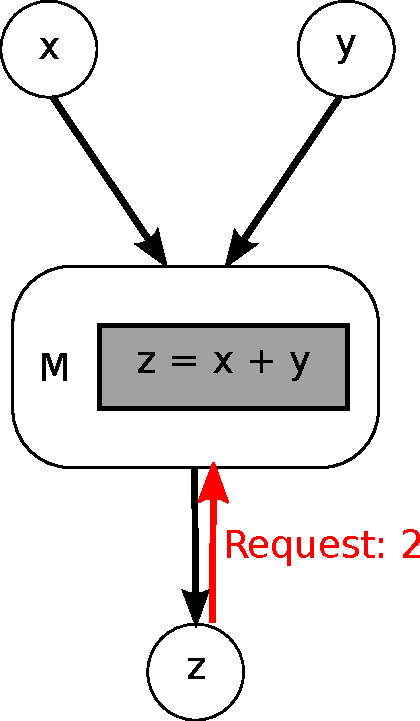
\includegraphics[height=5cm]{optim_use_1}
		\caption{The model agent receives a request.}\label{optim_use:1}
	\end{subfigure}
	\hfill
	\begin{subfigure}[b]{0.32\textwidth}
		\centering
		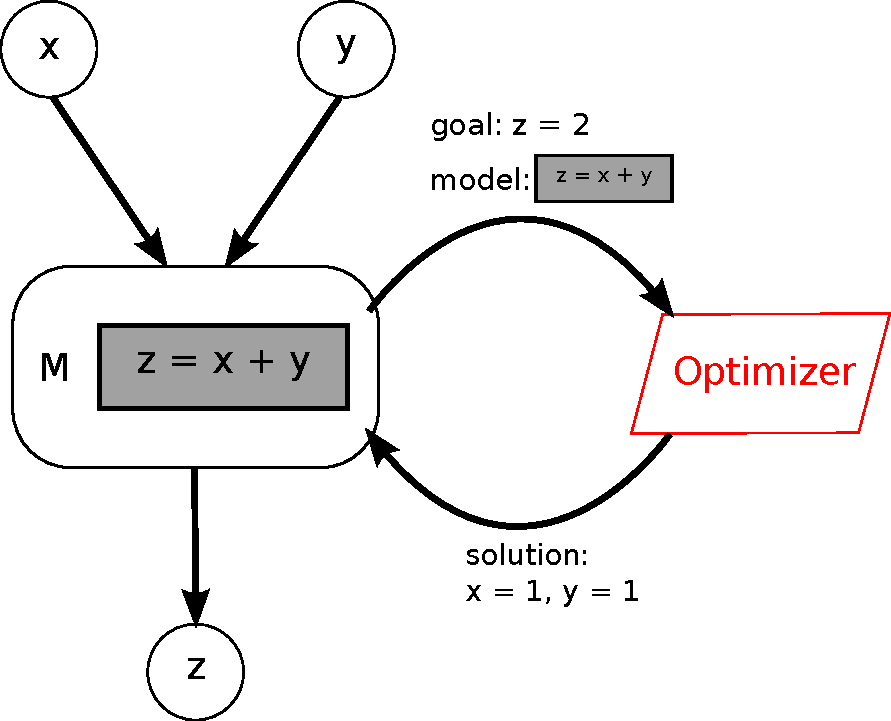
\includegraphics[height=5cm]{optim_use_2}
		\caption{The model agent resolves the request using an external optimizer.}\label{optim_use:2}
	\end{subfigure}
	\hfill
	\begin{subfigure}[b]{0.32\textwidth}
		\centering
		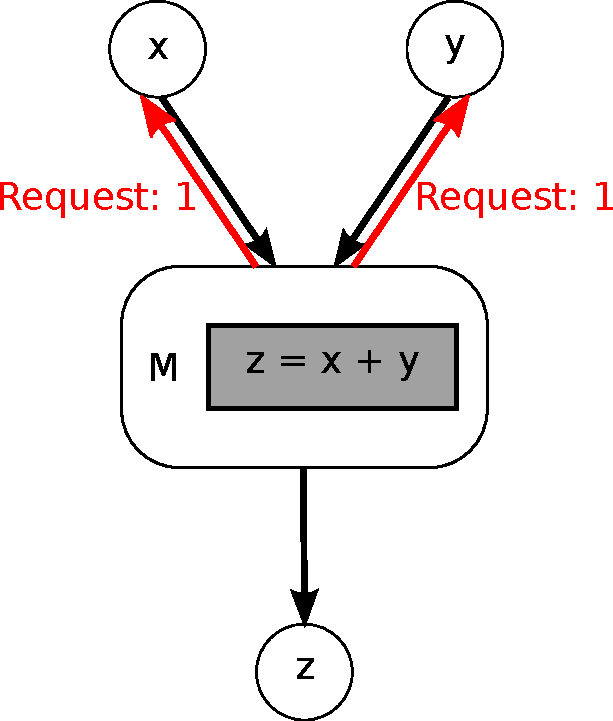
\includegraphics[height=5cm]{optim_use_3}
		\caption{The model agent transmits the new requests to its inputs.}\label{optim_use:3}
	\end{subfigure}
	\caption{Use of an external optimizer.}\label{optim_use}
\end{figure}

With this specificity in mind, let's now examine the behavior of the different agent types in the context of collective solving.

\subsection{Variable Agent}

During solving, a variable agent is susceptible to receive change requests from others agents. When a value agent receives a change request, it tries to change its own value  in order to accommodate the requester while trying taking in account the previous demands of the rest of its neighbors. To this end, the variable agent  uses an exploration strategy based on \emph{Adaptive Value Tracker} (AVT) \cite{Lemouzy_2011}. The AVT can be seen as an adaptation of dichotomous search for dynamic values. The main idea is to change value according to the direction which is requested and the direction of the past requests. While the value varies in the same direction, the variation delta is increased so the value varies more and more. As soon as the requested variation changes, it means that the variable went past the good value, so the variation delta is reduced.
This capability to take into account a changing solution allows the variable agent to continuously search for an unknown dynamic target value. This capability is required for the system to be able to adapt to changes made by the engineer during the solving process.

%While changing value based not on the value requested but on the direction can seem paradoxical, it must be recalled that, since no agent has a global view of the system, the requests made by the agents is often approximate, so the agents need to iterate many times. If the search space in large, the system could take time to converge towards the solution. By using a near-dichotomous strategy, we greatly accelerate this convergence.

[[Give analytical formulation of the AVT]]

One could wonder why the variable agent uses such a seemingly contrived method instead of just taking the requested value. It should be remembered that the variable agent can be connected to several parts of the problem and can receive contradictory requests from different origins over time (as we said, the case where the variable receives contradictory requests at the same time will also be studied later). Thus, the variable agent must have a way to take in account these contradictory requirements to find an adequate compromise. Moreover, until the system (or at least this part of it) has stabilized, the values requested has very little chance of being exact. The value can thus be considered as a  indication of the direction in which the requesting agent desire the variable to go. As the system stabilizes, the precision of the AVT is improved and the value of the variable is closer and closer to the exact correct value.

This behavior is summarized in algorithm \ref{algo_solving_variable}.

\begin{algorithm}
\caption{Collective Solving - Value Agent Behavior}
\label{algo_solving_variable}

	$v \leftarrow$ old value\;
	$v_r \leftarrow$ requested value\;
	$avt \leftarrow$ agent AVT \;
	
	\eIf{$v < v_r$}{
		$feedback \leftarrow$ INCREASE\;
	}{
		$feedback \leftarrow$ DECREASE\;
	}
	$v' \leftarrow$ $avt$.adjustValue($feedback$)\;
	
\end{algorithm}

\subsection{Model Agent}

The model agent is responsible for transmitting requests it received from its outputs to its inputs. To be able to translate the ingoing requests to its inputs, the model agent uses an external optimizer, as presented in introduction. When receiving a request from one of its outputs, the model agent calls the external optimizer, which provides it with the adequate inputs values corresponding to the request. The model agent then sends requests corresponding to these values to its inputs.
While the model agent can seem to be very simplistic, we will see in section [[REF]] how its 
behavior can be expanded to handle multiple problematic cases.

The behavior of the model agent is summarized in algorithm \ref{algo_solving_model}.

\begin{algorithm}
\caption{Collective Solving - Model Agent Behavior}
\label{algo_solving_model}

	$v_r \leftarrow$ requested value from output\;
	$M \leftarrow$ the internal model of the agent\;
	$O \leftarrow$ associated optimizer\;
	
	$\{v_r^i\} \leftarrow $O($v_r$, $M$) \tcp{get the input values estimated by the optimizer}\;
	\ForAll{$i \in$ input controlling agents}{
		send($i$, new Request($v_r^i$))\;
	}	
\end{algorithm}

[[Explain here ?]]
At the start of the section we stated that, since the internal model is a black box, the model agent cannot in itself perform the \enquote{bottom-up} translation from the values requested by its outputs to values to ask to its inputs, requiring an external optimizer to carry such task. While this is true at the start of the process, the model agent can at runtime observe the values returned by the model and make some estimations about its internal topology. We present now such a mechanism which can be integrated into model agents, capable of taking advantage of the functioning of the agent using simple black-box optimization techniques.

This mechanism integrates itself during the simulation behavior of the agent. Remember that, as presented in section \ref{simulation_model}, when receiving a new value from one of its input the model agent calls its internal model to recalculate the values of its outputs. At this step, instead of passing all the the agent can observe the impact of the variation of variation of the input on each output. We call \emph{correlation} between the input $i$ and output $o$ the variation of $o$ relative to the variation of $i$, calculated as $\dfrac{v_o^{t+1} - v_o^t}{v_i^{t+1} - v_i^t}$. This correlation can be seen as a local linear approximation of the partial derivative $\dfrac{\delta o}{\delta i}$.This correlation can then be used during solving to estimate the required changes from the inputs to satisfy a change requested by an output.\\
For example, suppose a model with one input $i$ and one output $o$. During simulating, the value of $i$ changes from 1 to 2. As a consequence the internal model provides a change of $o$ from -2 to -4. Thus the correlation between $i$ and $o$ is $\dfrac{-4 - (-2)}{2 - 1} = -2$. The output $o$ then sends a request to the model agent to take the value 4. The agent can estimate that for $o$ to take the value 4, $i$ needs to take the value $\dfrac{4}{-2} = -2$.
The complete formula when several inputs are involved in the calculus of $o$ is presented with the summary of the mechanism in algorithm \ref{algo_solving_internaloptim}.

\begin{algorithm}
\caption{Collective Solving - Internal Optimizer Algorithm}
\label{algo_solving_internaloptim}
	[[TODO]]\;
\end{algorithm}

We presented here a very simple learning mechanism for the agent to default when it is not provided with an external optimizer. This mechanism is voluntary simple and lightweight, in order to be applicable to a broad range of model topologies. While it is possible to make further refinements to improve its result, we believe that such needs are better covered by the use of external optimizers, which can be tailored for specific needs.

[[In Perspectives, remember to open on more complex techniques using contexts]]

\subsection{Output Agent}

Like for simulation, output agents have a similar role to variable agents during problem solving. However, as it depends of a model agent for its value, an output agent will simply transmits the requests it receives to its model, as summarized in algorithm \ref{algo_solving_output}.

\begin{algorithm}
\caption{Collective Solving - Output Agent Behavior}
\label{algo_solving_output}

	$v_r \leftarrow$ requested value\;
	$m \leftarrow$ the model agent responsible of the output \;
	
	send($m$, $v_r$) \tcp{forward the request to the model agent}\;
	
\end{algorithm}

\subsection{Constraint Agent}

With the objective agents, the constraint agents are the origins of the requests which are propagated into the system. The goal of a constraint agent is to ensure the constraint of which it is in charge is satisfied. To this end, the constraint agent calculates a target value for the constraint, estimates corresponding target values for its inputs and sends them as requests to the agents in charge of these inputs.

The problematic behind finding corresponding input values for the target value is similar to the one of the model agent of finding adequate inputs values from the outputs. As we said at the end of section \ref{modeling}, constraint agents (and objective agents) are similar to model agents in the fact that both have control of an \emph{internal model}. Thus, constraint agents can, in the same way than model agents, make use of an external optimizer to find adequate target values for its inputs. The only difference being that, instead of having a value requested by an output, the constraint agent estimates itself its own target value.\\
In the same way, constraint agents can use the same internal optimization mechanism than model agents, presented in algorithm \ref{algo_solving_internaloptim},  when not provided with an external optimizer.

The behavior of constraint agents is described in algorithm \ref{algo_solving_constraint};

\begin{algorithm}
\caption{Collective Solving - Constraint Agent Behavior}
\label{algo_solving_constraint}

	[[TODO]]\;
	
\end{algorithm}

It should be noted that, even when the constraint is satisfied, the constraint agent continues to send requests to its inputs. This behavior can be justified by several reasons.  First of all, the goal of the constraint agent is to ensure its constraint stays satisfied, so when the constraint is already  satisfied the constraint agent has interest in \enquote{pushing} its current value afar from the frontier.\\
The other reason is to help its neighbors agents keep a coherent view of their relations. Indeed, as the system is interactive, the designer can decide at any time to remove or change the constraint. As a consequence it is not possible for the agents to simply keep in memory the constraints they are linked to, as these informations can become obsolete at any time. A simple way to remedy to this situation is for the constraint to not assume the others agents will memorize its requirements and to keep sending them requests.

\subsection{Objective Agent}

Along with constraint agents, the objective agents are the origins of the requests which are propagated into the system. The goal of an objective agent is to improve the objective of which it is in charge. To this end, the objective agent iteratively estimates a new target value for its objective, finds the corresponding input target values and sends them as requests to the input agents.

Like the constraint and model agents, the objective agent can use an external optimizer to find the corresponding intput values, or can use the internal optimization mechanism presented in algorithm \ref{algo_solving_internaloptim}.

The behavior of objective agents is described in algorithm \ref{algo_solving_objective};

\begin{algorithm}
\caption{Collective Solving - Constraint Agent Behavior}
\label{algo_solving_objective}

	[[TODO]]\;
	
\end{algorithm}

It is interesting to note that the objective agent exhibits a behavior similar to the one of the constraint agent, but for slightly different reasons. While the constraint agent continuously sends requests in order to make its constraint safer and safer, the objective agent continuously send requests because it can never knows if it reached the best value for the objective it handles. An objective agent is essentially \enquote{blind}, as the objective is a black box, and must rely on the external optimizer (or the internal optimization mechanism) in order to improve it. Consequently, the objective agent never stops trying to find a better value. As with constraint agents, this mechanism is quite handy in the context of interactive optimization, as the designer can at any moment completely change the nature of the objective.

\section{Non-Cooperative Situations}

In the previous sections, we presented the basic agent behavior of our system. While this basic behavior could suffice in very simple test cases, it is not sufficient to handle the specificities of most continuous optimization problem configurations. In these situations, the nominal agent behavior (presented in the previous section) would lead to a suboptimal result.\\
Basing ourselves on the AMAS theory (presented in section \ref{amas_theory}), we can consider these configurations to be Non Cooperative Situations (NCS), as they represent a situation where, because of a shortcoming in the behavior of the agents, the system does not produces an adequate functionality (in our case, the optimization of the problem).\\
Consequently, we need for each NCS to provide the agents with specific mechanisms to:
\begin{compactenum}
\item detect occurring instances of the NCS
\item solve detected instances of the NCS
\item if possible, anticipate future instances of the NCS and avoid them
\end{compactenum}

Methodologically, by studying how the system handles specific problems with characteristics which are specific to continuous optimization (interdependencies, conflicting criteria \emph{etc.}), we identified several problematic configuration types, and defined different cooperation mechanisms for the agents that enable the system to correctly solve problems which exhibit these characteristics.

We will now present some additional mechanisms to handle some specific problematic cases we identified.

[[Explain the importance of modularity to handle different kinds of problems(external optims. etc.)
(=> cue to CPSP ?)
=> Maybe in conclusion of the chapter ?
]]

[[Dire pour chaque SNC à quelle catégorie elle appartient]]

\subsection{Conflicting Requests}

[[mettre les refs vers les travaux existants sur la criticité plutot dans la partie sur les CPSP ?]]

The first problematic configuration, and arguably the most obvious, is the one where an agent is in position of receiving simultaneous conflicting requests. This situation concerns every agent which is susceptible to receive requests: variable, model and output agents. This situation can be qualified as a \emph{Conflict} NCS, as the requesting agents ask for contradictory modifications of their environment.

When such an agent receives contradictory requests, it needs a way to select which request to apply and which request to reject. We can intuitively see how this decision should be based on the current state of the requesting agents. For example, when receiving requests both a satisfied and an non-satisfied constraints, a variable agent should favor the non-satisfied one. In order for the agents to be able to make this decision, we need to provide them with a way to compare the states of different agents.

To this end, we introduce a new mechanism based on a specific measure called \emph{criticality}. This measure represents the state of dissatisfaction of the agent regarding its local goal. Each agent is in charge of estimating its own criticality and providing it to the other agents\footnote{We do not concern ourselves with the problematic of trust here, each agent is assumed to provide the most trustful and accurate information without cheating or lying. The use of measures such as criticality in open and untrusted environments is in itself an interesting question to say the least.}. The role of this measure is to aggregate into a single comparable value all the relevant indicators regarding the state of the agent. Having a single indicator of the state of the agent is interesting as it simplifies the reasoning of the agents. In addition, this mechanism has the interesting property of limiting the informations transmitted to the others agents, which can be of interest in case of a distributed optimization where data privacy is an issue.
However the system designer has the difficult task to provide the agents which adequate means to calculate their criticality. Also, in specific cases, this information on the state of the agents is not sufficient to take the correct decision, as we will see in the following sections.

%%
In the proposed system, criticality is initially provided by constraint and objective agents and is propagated in the system through their requests.
Let's illustrate this with a constraint of the type \(g(X) \leq t\), with \emph{X} input of the constraint, \emph{g(X)} the constraint equation and \emph{t} the threshold under which the constraint is satisfied. The basic requirements regarding the criticality of this agent is to be low when the constraint is satisfied and high when the constraint is violated. Thus, the criticality of this agent is function of its current value and of the threshold.


\begin{figure}
	\centering
	\begin{subfigure}[b]{\textwidth}
	  \centering
	  \scriptsize
	  
		\[criticality_{t,\eta,\epsilon}(x)=
			\begin{cases}
				0		&\text{if \( x < \; t - \epsilon \) },\\
				-\gamma ( t - x - \eta ) ^ 2 / ( 2 ( \epsilon - \eta)) + \gamma ( t - x - \eta ) + \delta &\text{if \(t - \epsilon \leq \;x \leq \;t - \eta \)},\\
				\gamma (-t-x-\eta)^2/(2 \eta)+\gamma (-t-x-\eta) + \delta &\text{if \(t - \eta \leq \;x \leq \;t\)},\\
				1	&\text{if \( x > \; t \)}
			\end{cases}\]

		where\\
		$\gamma = -2/ \epsilon,$\\
		$\delta = -\gamma (\epsilon - \eta )/2,$\\
		$\text{and } 0 < \eta < \epsilon.$
	  \caption{Analytical formulation.}\label{crit_func}
	\end{subfigure}
	
	\begin{subfigure}[b]{\textwidth}
		\centering
		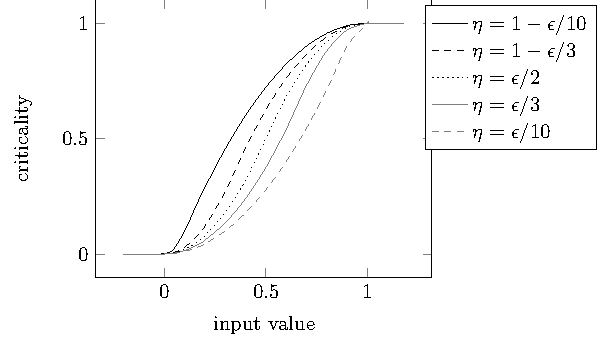
\includegraphics[]{./latex_figs/barrer-fig}
		\caption{Shapes of criticality function of threshold t = 1 for \(\epsilon=1\) and different \(\eta\).}\label{crit_shapes}
	\end{subfigure}
	
\caption{Criticality function of a constraint agent.}
\end{figure}

To compute it, we use the function defined on \figurename{} \ref{crit_func}. It takes as input \(x\), the current value of the constraint. It is parameterized by \(t\), the threshold, and by \(\eta\) and \(\epsilon\) that both regulate the shape of the function as seen on \figurename{} \ref{crit_shapes}. Its value always varies between \(0\) and \(1\).
The \(\epsilon\) can be adjusted by a domain expert if needed: the higher it is, the faster the constraint increases in criticality.
In our experiments, we used $\epsilon = 0.1$ and  $\eta$ was set to roughly a third of $\epsilon$, \textit{i.e.} 0.03.
This function allows a smooth transition between two states and provides several interesting properties: it is continuous, differentiable, requires few parameters, is computed quickly and is relatively easy to grasp.

[[Faire référence aux fonctions barrières présentées auparavant ?]]

\noindent The criticality of the other agents is determined as follow:

\begin{compactitem}
\item For objective agents: the criticality is set to an arbitrary constant value which must be lower than \(1\). In our experiments we settled for a value of \(0.5\). This translates the fact that, in the general case, an objective could theoretically always be improved, but is less important to satisfy than a constraint.
\item For variable, output and model agents: the criticality is set to the highest criticality among the received requests.
\end{compactitem}

When the system converges to a solution, it stabilizes at a point where the maximum of the criticalities of the agents is minimized.
%%

An illustration on this mechanism can be seen on \figurename{} \ref{NCS_1_conflicting_requests}. In this example, a variable agent (with a current value of 3) receives contradictories requests from an objective (decrease) and a constraint (increase). As the constraint is not satisfied, the criticality associated to its request (0.85) is higher than the one of the objective (0.5). As a consequence the variable agent selects the request of the constraint agent and increases its value.

\begin{figure}
	\centering
	\begin{subfigure}[b]{0.45\textwidth}
		\centering
		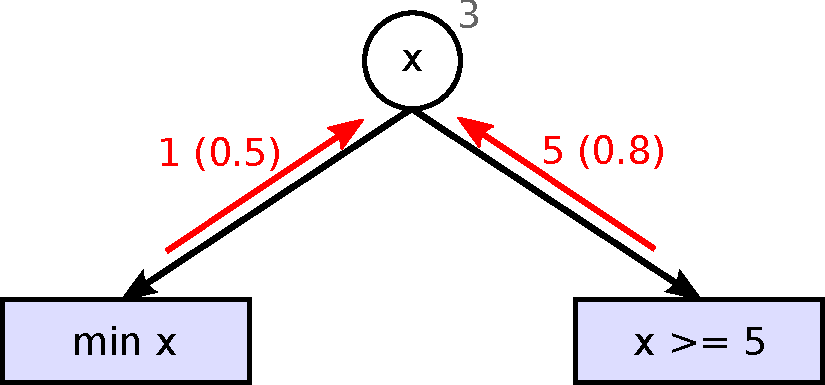
\includegraphics[width=\textwidth]{NCS_1_conflicting_requests_a}
		\caption{The criterions send their requests and current criticalities (in parenthesis).}\label{NCS_1_conflicting_requests_a}
	\end{subfigure}
	\hfill
	\begin{subfigure}[b]{0.45\textwidth}
		\centering
		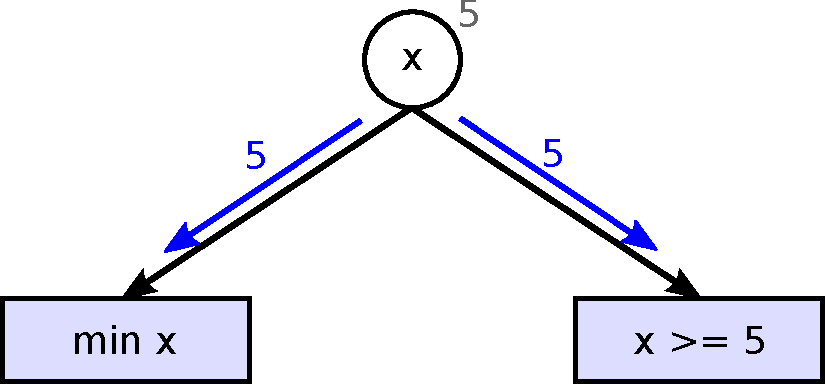
\includegraphics[width=\textwidth]{NCS_1_conflicting_requests_b}
		\caption{The variable agent selects the most critical request and responds accordingly.}\label{NCS_1_conflicting_requests_b}
	\end{subfigure}
	
\caption{Criticality mechanism (the criticality of the requests is indicated in parenthesis).}\label{NCS_1_conflicting_requests}
\end{figure}

\subsection{Cooperative Trajectories}

\subsubsection{For Model Agents}

This NCS can be seen as an extension of the previous one (conflicting requests). It occurs when a model agent receives requests from its outputs which lead to contradictory changes on its inputs (\emph{Conflict} NCS). We presented in the previous section how using \emph{criticality} the model agent could discriminate between the requests by choosing to satisfy the most critical. However, in the specific case of the model agent, this mechanism is not the most efficient. Let us take a simple example.

Suppose the following problem:

\begin{align*}
\text{Minimize } &x\\
\text{subject to } &y > 0\\
\end{align*}
Where $x,y$ are outputs of the model $M(a,b)$ defined as
\begin{align*}
x = &10a + b\\
y = &a + 10b\\
\end{align*}

Using conflicting requests mechanisms, the model agent $M$, upon receiving requests coming from the objective and constraint agents, would choose to fully satisfy the most critical request, disregarding completely the other. In this example, if the request of the objective agent is the most critical, the model agent would ask $a$ and $b$ both to decrease, and would ask them both to increase if the constraint agent request was the most critical.\\
However we can easily observe how, in this specific problem, the input variables $a$ and $b$ has different impacts on the objective and the constraint. A variation of 1 for the variable $a$ will change the objective by 10 and the constraint by 1, while a variation of 1 for the variable $b$ will have the inverse effect.\\
This observation leads to a third possibility: trying to satisfy both requests at once by propagating each request to the input agent(s) which is (or are) the most \enquote{influential}[[NOTE: try to find a synonymous, influence will be used elsewhere]] for each request. Doing so allows a most efficient exploration of the search space by improving several criteria at once.

[[Drawing of cooperative trajectory search space in 2D]]

Let $M(I,O)$ be a model agent with a set of inputs $I$ and a set of output $O$.

Let $\{r = <\Delta_{o_{\in O}}^{r}, crit>\}$ be a set of  requests received for outputs $\{o\} \in O$, where $\Delta_{o}^{r}$ is the variation of output $o$ requested by $r$ and $crit$ the criticality of the request. By hypothesis, at most one request can concerns the same output.
Using an external optimizer, the agent obtains for each $r_k$ a set of corresponding input variations $\{\Delta_i^{r_k}\}_{i \in I}$.

For each input $i$ of the model, we need to select a variation.
First of all, we only keep the requested variations with the maximum criticality:  $\{\Delta_i^{r_{max}}\} \leftarrow \{\Delta_i^r : crit_r = max \{crit_{r \in R}\}\}$.
If $|\{\Delta_i^{r_{max}}\}| =  1$, then the agent knows which variation to request to the input agent.

Otherwise, the model agent will discriminate using the relative influence [[it learned | given by the analyser]] of the input on the outputs concerned by the requests: 
$\Delta_i^* \leftarrow \left\{ \Delta_i^{r_{max}} : r_{max} = argmax \dfrac{inf_{i,o_{r_{max}}}}{\sum \limits_{i \in I} inf_{i,o}} \right\}$

If at this step $|\Delta_i^*| >1$ [[then what?]]. Otherwise the unique $\Delta_i^*$ is selected.

\begin{algorithm}
\caption{Cooperative trajectory - Model agent}
\label{algo_cooperative_trajectory_model}

	\ForEach{$i \in I_M$}{
		 $\{\Delta_i^{r_{max}}\} \leftarrow \{\Delta_i^r : crit_r = max \{crit_{r \in R}\}\}$\;
		 \eIf{$|\{\Delta_i^{r_{max}}\}| = 1$}{
		 	$\Delta_i^{r_{max}}$ is the variation requested to the input\;
		 }
		 {
			$\{\Delta_i^*\} \leftarrow \left\{ \Delta_i^{r_{max}} : r_{max} = argmax \dfrac{inf_{i,o_{r_{max}}}}{\sum \limits_ {i \in I} inf_{i,o}} \right\}$\;
		 }
	}

\end{algorithm}

\subsubsection{For Variable Agents}

We have seen in the previous section how it could be possible in some cases to propose an more efficient exploration of the search space by making model agents selectively propagate requests based on the influences[[OTHER TERM ?]] of theirs inputs on theirs outputs. This mechanism based itself on the fact that all the requests pass by a model agent, which is able to \enquote{dispatch} the requests to different inputs.\\
However, if we take the example problem, we can reformulate it as the following equivalent problem:

\begin{align*}
\text{Minimize } &10a + b\\
\text{subject to } &a + 10b > 0\\
\end{align*}

Using this new formulation, no model agent is create during the MAS transformation of the problem, but the underlying problem between cooperative trajectories still exists but with an additional difficulty. As we already said, in order to be able to scale with the complexity of the problem, each agent must keep a local view. Consequently, the criteria agents are not aware of each others, and neither are the variable agents.\\
We will now show how the variables agents can become aware of the NCS and coordinate to solve it without communicating with, or even acknowledging, each other.

\subsection{Cycle Solving}

\subsection{Hidden Dependencies}

\subsection{Asynchronous Requests}

\section*{}
The most important point is that each agent only has a local strategy. No agent is in charge of the optimization of the system as a whole, or even of a subset of the other agents. Contrary to the classical MDO methods presented earlier, the solving of the problem is not directed by a predefined methodology, but by the structure of the problem itself. The emerging global strategy is unique and adapted to the problem.

\begin{algorithm}
\caption{Agents Behaviors}\label{agent_algo}

\SetKwProg{Bv}{behavior of }{}{}

\Bv{Model Agent}{
	\Repeat{resolution end}{
		analyze received messages\;
		\If{received new information messages}{
	        recalculate outputs\;
	        inform depending agents\;
	    }     
		\If{received new requests}{
	        use optimizer to find adequate inputs\;
	        propagate requests to input agents\;
	   }
	}
}

\Bv{Variable Agent}{
	\Repeat{resolution end}{
		analyze received messages\;
		\If{received new requests}{
	       select most important\;
	       adjust value\;
	       inform depending agents\;
	    }
	}
}

\Bv{Output Agent}{
	\Repeat{resolution end}{
		analyze received messages\;
		\If{received new information messages}{
	        update its value\;
	        inform depending agents\;
	    }      
		\If{received new requests}{
	        select most important\;
	        transmit selected request to model agent\;
	    }
    }
}

\Bv{Constraint/Objective Agent}{
	\Repeat{resolution end}{
		analyze received messages\;
		\If{received new information messages}{
	        update its value\;
	        use optimizer to find adequate inputs\;
	        send new requests to variable/output agents\;
	    }
	}
}

\end{algorithm}

\chapter{Extending the Multi-Agent System for Uncertainties}

We have seen in section \ref{SOA_uncertainties} how uncertainties can be a major concern in real-life optimization. We have also seen how several types of uncertainties existed and needed to be taken into account. Moreover, complex optimization problems can involve several teams concerned with different disciplines, each of which with its own practices regarding how to manipulate uncertainties, making difficult to study the impact of uncertainties across disciplines.

In this chapter we present a way to alleviate this burden by having the agents automating the uncertainty propagation in the system.

The difficulty is twofold:
\begin{compactitem}
\item \textbf{How do the agents handle uncertainties ?}
How does a model agent calculate the uncertainties on its outputs from the uncertainties of its inputs and its internal model ? How does a constraint agent can handle a probabilistic constraint ?

\item \textbf{How do the agents combine heterogeneous uncertainties modeling ?}
How can a model agent handle inputs with different uncertainties modelings ?
\end{compactitem}

To answer these difficulties we will present a general mechanism inspired by the one we used with external optimizers, which is based on the use of encapsulated external tools to apply the domain-specific expertise.

\section{From Deterministic Optimization to Optimization under Uncertainties}

[[Reformulation d'un probleme d'optim] -> cf these_Vicent_Baudoui_Optimization_robuste]]

We previously explained that uncertainties can be present at several levels in the optimization problem. We consider here the two following types of uncertainties:
\begin{compactitem}
\item \textbf{Variable uncertainties}, which are brought by the fact that we cannot perfectly control the value which will be effectively assigned by the design variable.
\item \textbf{Model uncertainties}, which represent the limited precision of the models.
\end{compactitem}

Taking in account these uncertainties leads to a modification of the criteria formulation. Indeed, the constraint $x < 10$ makes sense in the context of deterministic optimization, but not so much when the value of $x$ is uncertain. Is the constraint satisfied when $x$ is an uncertain value, for example represented by an interval ranging from 8 to 12?\\
One can instead propose the following probabilistic constraint $P(x < 10) > 90\%$, which can still be evaluated when manipulating uncertain values. It is possible to propose others criteria formulations manipulating uncertain values, for example one could consider a deterministic constraint concerning the mean of an uncertain variable. Usually, constraints are expressed in a probabilistic form, while objectives use the mean of the variables[[NEED TO REF THIS ?]].

[[Give an example of transformation of a deterministic problem to a non deterministic one]]

\section{Manipulating Uncertain Values}

[[Bien expliquer que la surcharge des operateurs ne concerne que les agents, et non pas le contenu des boites noires]]

Taking in account uncertainties requires modifications at several levels. The most obvious concerns the data structure. On the deterministic version, the data exchanged by the agent were simply real values \footnote{With the obvious limitation of the representation of real numbers on a machine.}. To be able to exchange uncertain values, the agents require a more complex data structure.

As we presented earlier, there are many ways to represent uncertainties, each of them having specific requirements. For example, an interval representation requires two values, the minimum and maximum boundaries, while an uncertainty expressed by a set of measures obtained with Monte Carlos experiments can require the storage of hundreds of thousands points. As we want to maintain the possibility for the designers to choose how they represent uncertainties, we need to provide an abstraction for the agents to be able to consistently handle uncertain values whatever the specific representation [[CORRECT ENGLISH?]].

To this end, we specified the minimum set of operations the agents require. To be able to manipulate an uncertain value, an agent needs to be able to :
\begin{compactitem}
\item obtain the mean of the value (or at least a representative value).
\item obtain the standard deviation of the uncertainty.
\item draw a random value following the law represented by the uncertainty.
\item obtain the cumulative probability of a value (\emph{i.e.} for a given value $t$, what is $P(X < t)$) 
\item obtain the inverse cumulative probability (for a given probability $p$, what is $t$ for which $P(X < t) = p$) associated with the uncertainty).
\end{compactitem}

Any uncertainty representation which can provide these five informations can be used by the system. All the designer needs to do is to provide the module which implements these operations\footnote{The reader familiar the concepts of object-oriented programming and interface implementation will have no difficulty to guess how the process is done in our prototype}.

Let us see how one can provides these information regarding two drastically different modelings: intervals and Monte Carlo experiments.

\paragraph{Intervals Representation}

As the reader knows, an interval representation consist of a lower and upper boundaries. It can be considered as an uniform law, with all the values between the boundaries considered as equally likely. Suppose $l$ and $u$ the boundaries of our uncertainty, we can obtain the required informations using well-known formulas for the uniform law.

\begin{compactitem}
\item the mean can easily be obtained as $\dfrac{u + l}{2}$.
\item the standard deviation is $\sqrt{(u - l)^2 / 12}$.
\item the drawing of a random value consists of drawing a value between $l$ and $u$ using an uniform law, which presents no difficulty.
\item the cumulative probability of $t$ is calculated as $P(X < t) =
			\begin{cases}
				0	&\text{ if t < l}\\
				 \dfrac{t - l }{u - l}	& \text{ if } l < t < u\\
				1	&\text{ if t > u}
			\end{cases}$
\item the inverse cumulative probability of $p$ is obtained as $t = l + p (u - l)$.
\end{compactitem}

As we can see, for a simple representation as intervals the required informations can be obtained very easily.

\paragraph{Monte Carlo Experiments}

The Monte Carlo Experiment is not an uncertainty law \emph{per se} but a series of random drawings to obtain experiment points. If the number of drawings is big enough, then the series can provide an adequate information about the uncertainties governing the variable. Suppose $\{x_n\}$ a series of $n$ drawings over $x$. We suppose the values to be ordered (that is, $x_i < x_j$ 

\begin{compactitem}
\item the mean can be obtained with $\dfrac{\sum_n{x_n}}{n}$.
\item the standard deviation is obtained by first calculating the variance using the formula $Var(X) = E(X^2) - E(X)^2$ (possible as we can calculate the mean), then taking the square root to obtain the standard deviation.
\item the drawing of a random value consists of drawing a value $i$ between $1$ and $n$ and returning the corresponding point $x_i$
\item the cumulative probability of $t$ is calculated as  $P(X < t) = \dfrac{|\{x_i, \forall x_i < t\}|}{|\{x_n\}|}$ (where $|\{x\}|$ is the cardinality of the set $\{x\}$), \emph{i.e.} the number of elements lower than $t$ divided by the total number of elements.
\item the inverse cumulative probability of $p$ is obtained as $ t = $ [[TODO]].
\end{compactitem}

Even with very specific, non-analytical representation of uncertainties such as datasets from Monte Carlo experiments, we can provide the needed informations without much hassle.

Now that we have defined a common set of operations common to all the uncertainties representations, we can adapt the agents behavior in order to handle them. Such \enquote{uncertainty container} can be associated to variables to represent uncertain values, or to models, indicating uncertainties concerning the underlying model.

For example the designer can estimate that, due to physical limitations, the value of a design variable $x$ cannot be exactly be controlled and will always suffer from an imprecision of +/-0.1 around its assigned value. He can model the uncertainty around the variable with an interval. If he decides to arbitrarily initialize the variable at the value 8, the uncertain value of $x$ will then be [7.9; 8.1].

If the designer observe that the real-world process represented by a specific model tends to produce outputs whose values imprecision can be accurately modeled by a normal distribution, he can associate the normal distribution uncertainty to the model. For example the model $y = 2x$, upon the reception of the information $x = 1$, will produce an uncertain value $y$ with a mean of 2 and a variance corresponding to the associated normal law.

We have now seen how the agents can manipulate uncertainties in isolation. But these mechanisms do not allow the agents to propagate uncertainties in the system. Indeed, if we take our two previous examples, what if the variable $x$ ,associated with an interval uncertainty, is assigned in input of the model $y = 2x$, following a normal distribution? The model has no mechanism to handle uncertainties \emph{received on its inputs}, but these uncertainties must be taken into account as they surely have consequences on the uncertainties of its outputs.\\
The difficulty here is twofold. Not only the model agent must be able to take in account the uncertainties provided by its inputs in addition to its own uncertainty, but it must be able to do so even with uncertainties of different kinds (in our example, interval and normal distribution). We will now present a generic mechanism using \emph{uncertainties propagators} which allows to solve both problems at once.

\section{Uncertainties Propagators}

[[Need to illustrate how the propagator is used at runtime (diagram)]]

In the same way we encapsulated expert knowledge on numerical optimization using external optimizers, we propose to encapsulate the knowledge related to the propagation of uncertainties into dedicated modules we call \emph{uncertainties propagators}. While external optimizers are used by the agents to solve local optimization problems, the uncertainties propagators are used by the agents to propagate the uncertainties associated with their inputs and model into uncertainties on their outputs.

The role of an uncertainties propagator is to determine the uncertainties associated with the outputs values of the model based on:
\begin{compactitem}
\item the model itself
\item the uncertainty associated with the model
\item the input values
\item the uncertainties associated with the inputs
\end{compactitem}

As the outputs values cannot be determined by simply evaluating the (deterministic) model, the agent in charge of it will delegate the whole evaluation process to the uncertainties propagator when working with uncertainties. From the agent point of view, an uncertainties propagator is a black box function taking uncertain input values and an uncertain model, and producing uncertain outputs values.

\begin{figure}
\center
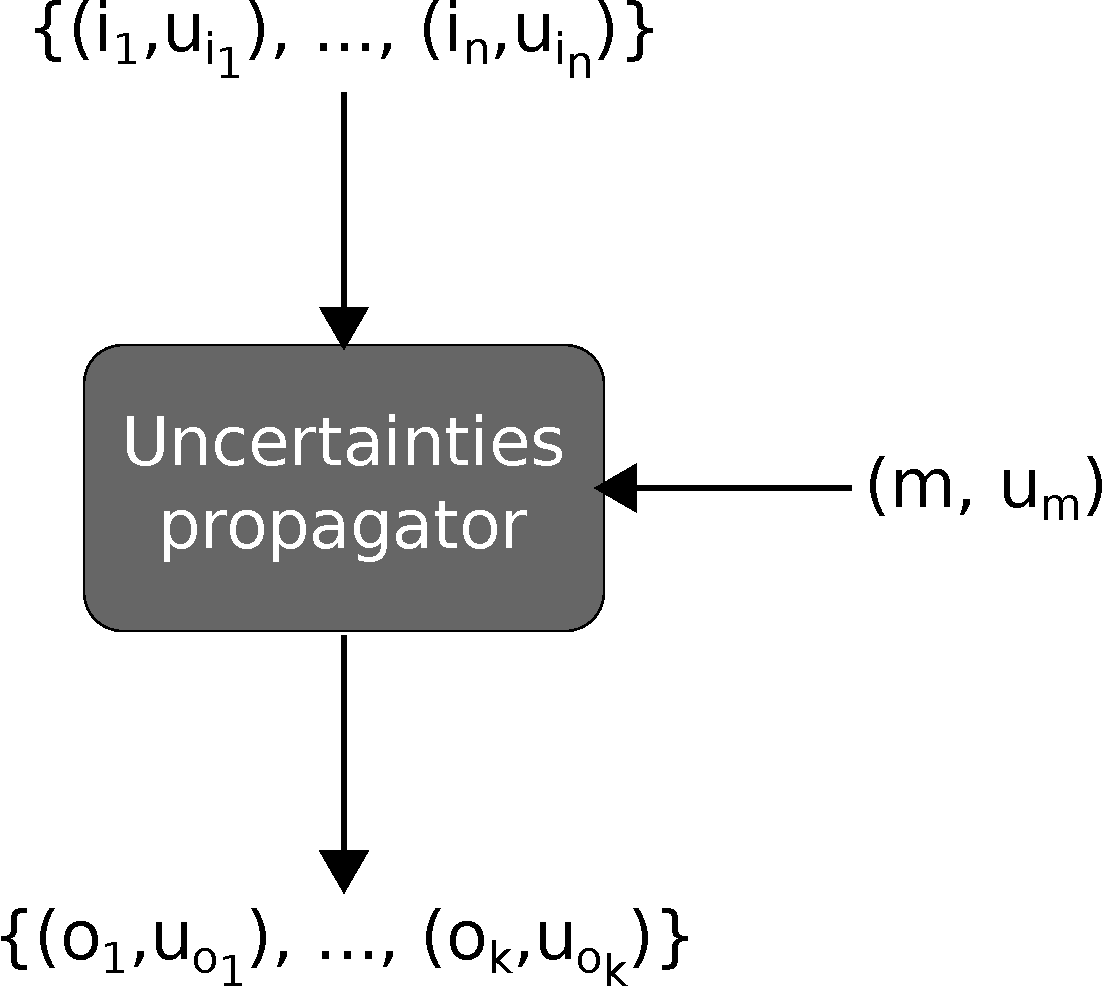
\includegraphics[width=0.4\textwidth]{uncertainties_propagator}
\caption{Uncertainties propagator as a black box function.}\label{uncertainties_propagator}
\end{figure}

\figurename{} \ref{uncertainties_propagator} illustrates the representation of an uncertainties propagator from the point of view of an agent. The uncertainty propagator is a black box. The $(i_j, u_{i_j})$ represent the $n$ uncertain input values of the model (the $i_j$ corresponding to the mean value of the input and $u_{i_j}$ to the associated uncertainty). The model itself $m$ is also provided along with its associated uncertainty $u_m$. Based on the inputs and the model (and their uncertainties), the uncertainty propagator returns the $(o_j, u_{o_j})$ represent the $k$ uncertain output values produced.

This approach shows several advantages. First it allow to keep the functioning of the agents nearly untouched, which in itself is a good sign. Handling uncertain values can be deemed to be an orthogonal concern to the previous ones, and orthogonal concerns should lead to orthogonal changes. Thus this modification of our system to handle uncertainties show that \emph{our modeling is flexible and can be extended easily}.\\
This approach also permit to reduce the work of the designers, which only need to \emph{define the needed propagators once and reuse them} on several problems. This aspect is particularly important as defining a correct way to propagate uncertainties across different disciplines can be an extensive work involving experts from different domains. Providing a way to encapsulate the result of this work in a reusable component leads to a more efficient work process (this concern is especially recognized by software engineers, which created the well-known acronym: DRY - \enquote{Don't Repeat Yourself}).\\
Finally, by strictly encapsulating the required knowledge, we provide a highly modular and adaptable mechanism. \emph{If the needs regarding the modeling of the uncertainties changes, the consequences on the problem are limited solely to the uncertainties representation and/or propagators}. For example, if a designer needs to change the uncertainties associated with a model, he only has to change the uncertainty representation of the model and to use the appropriate propagator (or create it if no adequate propagator already exists).

[[Dire que les propagateurs peuvent être très génériques et très réutilisables, ou au contraire extremement specifiques et adhoc => transition sur la partie suivante]]



\subsection{Examples of Propagators}

\section{Conclusion on Uncertainties Handling}

We have seen how the agents can automatically propagate uncertainties in the system, relieving the designers of a part of the burden.\\
This extension to our modeling allow to take in account not only values but uncertain values, that is, values with an associated uncertainty representation. As the exact representation does not concern the agent, these uncertainties are mostly handled as black boxes. In a similar way to how they use optimizers to propagate requests with black box models, internal model agents can use uncertainties propagators to locally propagate uncertainties. In this regard, uncertainties propagators (as well as external optimizers) can be seen as a way to extend the capabilities of the agents provided by the users.

While this mechanism require for the users to provide the uncertainties propagators, it has the advantage that this specific effort has to be done only once, as the resulting propagator can be reusable at will. In this way it can greatly reduce the time different teams need to spend together to overcome the difficulties induced by different working practices. It also open the possibility of propagators libraries, which can be shared and imported as needed.

A note of warning however, the representation of uncertainties is inherently imprecise. In the same way that the modeling of a system contains imprecision, so does the modeling of the uncertainties used to represent this very same imprecision (and so would do the uncertainties used to represent the imprecision on the uncertainties...). Like discussed before, this imprecision is an inherent limitation of the real world. As the uncertainties modeling is in itself factor of uncertainties, it follows that the transformation between two different uncertainties representations will in itself contains some part of imprecision (if only because the passage from one representation to another can lead to information loss, \emph{e.g.} passing from a normal law to an interval modeling).\\
This problematic is not specific to our technique and is indeed  present all the same if the uncertainties propagation is done \enquote{manually}. But it is worth reminding, as this complete automation of the propagation could hide it from the mind of the designer.

As a remark we have seen how, by overloading some common mathematical operators, it was possible for the agents to manipulate uncertain values as if they were simple numerical values. Such work could be possibly done with complex numbers, matrix or others, arbitrarily complex, data structures, as long as the corresponding overloaded operators are provided.